%! TEX program = xelatex
\documentclass[12pt,a4paper]{article}
\usepackage[a4paper,margin=1in]{geometry}
% \usepackage[localfonts=true]{tenth}
\usepackage{tenth}

% Load pre-defined page numbers of diagrams
%% Generated by ipescript page-labels drawings.pdf
%% Do not edit
\newcommand{\ipeFigPetersen}{1}


\renewcommand{\pageheader}{\sffamily\textsb{หัวข้อที่น่าสนใจ} — โดยคุณ}
\title{หัวข้อที่น่าสนใจ}
\author{ชื่อจริง และนามสกุล}
\date{}

\begin{document}

\maketitle
\thispagestyle{titlepage}
\setstretch{1.3}

\section*{หัวข้อแรก}

\begin{theorem}
    สำหรับ $n \in \mathbb{Z}$ ใด ๆ จะพบว่า $n$ เป็นจำนวนคู่\hrsp{}\uline{ก็ต่อเมื่อ} $n^2$ เป็นจำนวนคู่ 
\end{theorem}

\begin{definition}
    กราฟต่อไปนี้มีชื่อเรียกว่า Petersen Graph
    \begin{center}
        \includegraphics[page=\ipeFigPetersen,scale=0.8]{diagrams/drawings.pdf}
    \end{center}
\end{definition}

\begin{question}
    สามเหลี่ยมใด ๆ ในปริภูมิยูคลิด (Euclidean space) จะมีมุมภายในรวมเป็นเท่าใด?
\end{question}

\begin{theorem}
    เอกลักษณ์อนุกรมเรขาคณิตต่อไปนี้เป็นความจริง
    \[
        1^1 + 1^2 + 1^3 + \ldots + 1^n = n \tag*{\qedhere}    
    \]
\end{theorem}

{\elseries\lipsum[1]}

{\ltseries\lipsum[2]}

{\mdseries\lipsum[3]}

{\mbseries\lipsum[4]}

{\sbseries\lipsum[5]}

{\bfseries\lipsum[6]}

{\ebseries\lipsum[7]}

\end{document}
